\subsubsection{Gaussian Mixture Models}
\label{sec:GMM}
One of the most common distributions is the Gaussian distribution $ \mathcal{N}(\mu,\sigma)$. Sometimes this model is not quiet enough to capture the underlying distribution. In such cases can a mixture of Gaussian distributions be created to fit a underlying distribution. This principal is shown in figure \ref{fig:mixturemodel}. 

\begin{figure}[H]
\centering
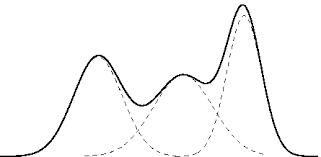
\includegraphics[scale=0.5]{billeder/MixtureModel}
\caption{Gaussian Mixture Model Principe}
\label{fig:mixturemodel}
\end{figure}

This method can be generalized up in a multidimensional space, to fit the feature space. In a multidimensional model we introduce the covariance matrix $\Sigma$ that like $\sigma$ gives the deviation of a Gaussian model. The Gaussian mixture model can therefore be described as: 

\begin{equation}
 P(x) = \sum\limits_{k=1}^K{ \Pi_k \mathcal{N}(x|\mu_k,\sigma_k) }
\label{eq:mixturemodel}
\end{equation}

Where $\Pi_k$ is a weight called the mixture parameter, that is used to differentiate the individual Gaussian distributions in the model. knowing this we can also describe the mixture model from equation \ref{eq:mixturemodel} as: 

\begin{equation}
 P(x) = \sum\limits_{k=1}^K{ P(k) P(x|k) }
\label{Eq:mixturemodel}
\end{equation}

In order to use a the mixture model, the different distributions must first be found. This topic will be discussed in section \ref{sec:k-means} and \ref{sec:EMAlgorithm}

\subsubsection{k-means Algorithm}
\label{sec:k-means}

One way of finding groupings of data, in the feature space, is by using the k-means algorithms. This algorithm tries to split the data in k groups. This is done by following 4 three step iterating proses. 

\begin{enumerate}
  \item Initialize means: Select k random mean values in the feature set. 
  \item Assign responsibility: For each point, find the closest mean points and make it responsible for that point.
  \label{step:iteratemeans} 
  \item Calculate new mean: Move each mean point to the mean value of the cluster of points the mean is responsible for. 
  \item Continue whit step \ref{step:iteratemeans}, till no change in points. 
\end{enumerate}

On figure \ref{fig:kmeans} is illustrated how the k-means in 6 iterations split the data up in 3 clusters.

\begin{figure}[H]
\centering
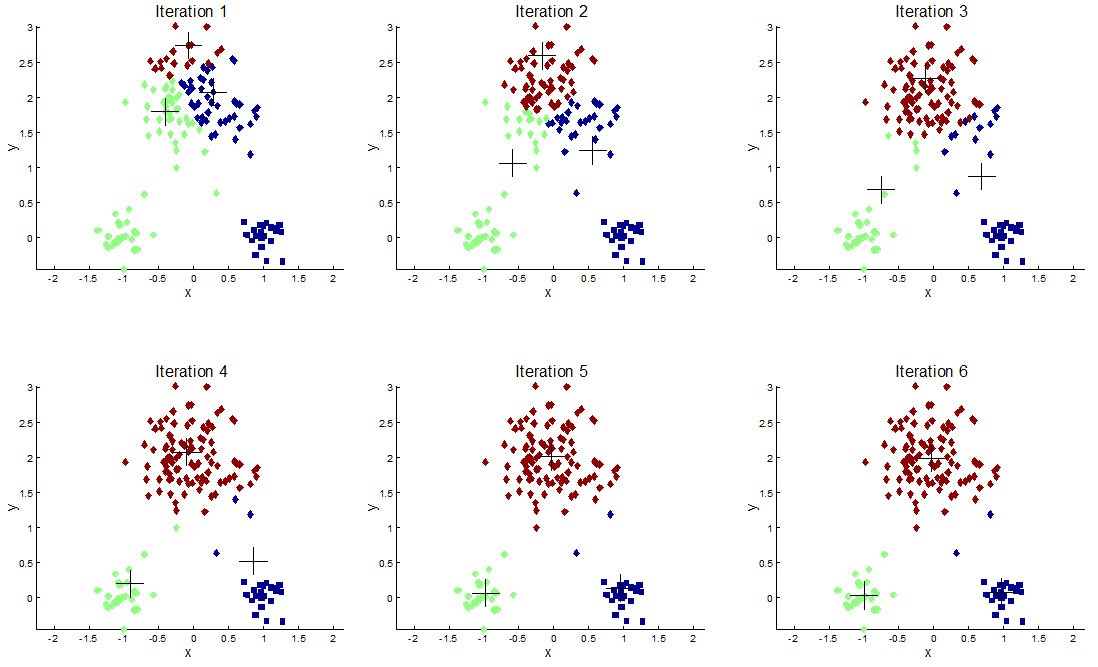
\includegraphics[scale=0.6]{billeder/kmeansclustering}
\caption{K-means used on a data set}
\label{fig:kmeans}
\end{figure}

The result of this proses will differ depending on the initial mean guesses. This is especially the case is there is no natural groupings in the dataset. In this case the algorithm will still split up the data in k clusters there are side by side. This is illustrated on figure \ref{fig:badkmeans}, where the k-means algorithm tries to cluster points distributed uniformly on a circle, in 7 clusters. 

\begin{figure}[H]
\centering
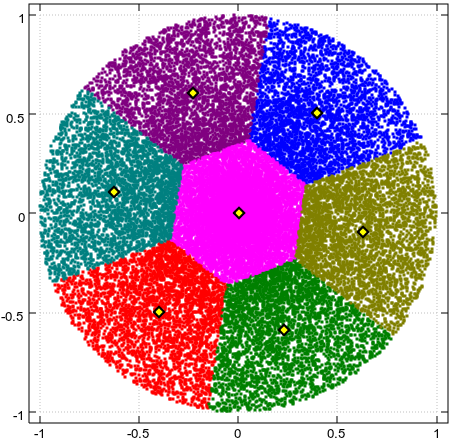
\includegraphics[scale=0.5]{billeder/CircleClusters}
\caption{K-means used on points distributed uniformly on a circle}
\label{fig:badkmeans}
\end{figure}

\subsubsection{EM Algorithm For Gaussian Mixture Models}
\label{sec:EMAlgorithm}

As discussed in section \ref{sec:GMM} it is important to have a method of finding the best Gaussian distributions in the data set to create a good mixture model. The best Gaussian Mixture Models that fits the data can be described as optimising equation \ref{eq:maxgmm}.

\begin{equation}
 L(x) = \sum\limits_{n=1}^N{\log{\sum\limits_{k}^K P(k) P(x_n|k) }}
\label{eq:maxgmm}
\end{equation}

To find the maximum of equation \ref{eq:maxgmm}, we find the differentiated and set et equal zero. 

 \begin{equation}
 \frac{\partial L(x)}{\partial{\mu_k}} = 0
\label{eq:partialzero}
\end{equation}

From equation \ref{eq:mixturemodel} and \ref{eq:maxgmm} the following optimisations equations can be found: 

\begin{equation}
 N_k = \sum\limits_{k}^K P(k|x_n)
 \label{eq:em1}
\end{equation}
\begin{equation}
 P(k)= \Pi_k = \frac{N_k}{N}
 \label{eq:em2}
\end{equation}
\begin{equation}
 \Sigma_k= \frac{1}{N_k} \sum\limits_{n}^N{ P(k|x_n) (x_n -\mu_n)(x_n-\mu_k)^\intercal}
 \label{eq:em3}
\end{equation}
\begin{equation}
 \mu_k= \frac{1}{N_k} \sum\limits_{n}^N{ P(k|x_n) x_n}
 \label{eq:em4}
\end{equation}

The variable $N_k$ can be seen as the effective number of samples in a cluster, and $N$ is the total number of samples. The $P(k|x_n)$ term can be seen as the responsibility a center point has for that point. Unlike the K-means algorithm the all center points are responsible for all points, but the level of responsibility is different from center point to center point. To find the optimal center points $\mu_k$, and there deviations $\Sigma_k$ the EM algorithm can be used. This is based on a the idea of a E-step, called the estimation step, and a M-step called the maximisation step. Much like the k-means does this also have 4 iterative steps. 


\begin{enumerate}
  \item Initialize Parameters: Select k random values for $\mu_k$ , $\Sigma_k$ , $\Pi_k$
  \item E-Step: Update the responsibility by using Bayes' theorem stating: 
 \begin{equation}
 	P(k|x) = \frac{P(x|k) P(k)}{P(x)} = \frac{P(x|k) P(k)}{\sum\limits_{k}^K{ P(x|k) P(k)}}
 \end{equation}
  
  \item M-Step: Maximize the Gaussian mixture model parameters by using equations \ref{eq:em1}, \ref{eq:em2}, \ref{eq:em3} and \ref{eq:em4}. 
  
  \item Continue whit step 2, till no change in Gaussian mixture model parameters. 
\end{enumerate}

Like the k-means algorithm does this algorithm also map a predetermined number of Gaussian distributions to the dataset. The optimal amount must be found though exploration. On figure \ref{fig:UGMM} we see how the EM algorithm has been used to map 3 Gaussian mixture model to a dataset. 

\begin{figure}[H]
\centering
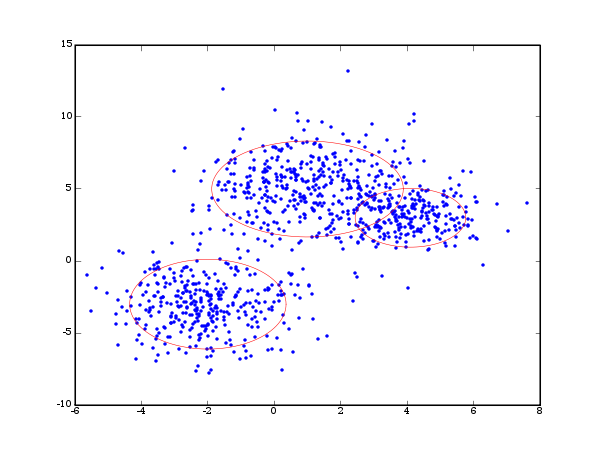
\includegraphics[scale=0.5]{billeder/UGMM}
\caption{EM Algorithm Used On Data To Create GMM}
\label{fig:badkmeans}
\end{figure}

Like for the k-means the initaial start estimates for the mean value is important for a good result, and a fast execution time. A normal approach is to use the k-means algorithm first, and use the final means as the start estimate in the em algorithm.

\subsubsection{Unsupervised Gaussian mixture model}
 hvad er det\\
 
 hvordan er det brugt i projektet\\
 
 del resultat \\
 
\subsubsection{Supervised Gaussian mixture model}
\label{sec:EMGMM}

 hvad er det\\
 
 hvordan er det brugt i projektet  
 
 del resultat 

%------------------------------------------------